\documentclass[11pt,a4paper, titlepage]{article}
\usepackage[utf8]{inputenc}
\usepackage[T1]{fontenc}
\usepackage[left=2cm,right=2cm,top=2cm,bottom=2cm]{geometry}
\usepackage{pdflscape}
\usepackage[spanish, activeacute]{babel}
\usepackage{amsmath}
\usepackage{amssymb,amsfonts,textcomp}
\usepackage{color}
\usepackage{array}
\usepackage{hhline}
\usepackage{rotating}
\usepackage{graphicx}
\usepackage{lipsum}% dummy code
\usepackage{colortbl}
\usepackage{subfigure} % subgráficos
\usepackage{xtab}
\usepackage{longtable} % para tablas largas
\usepackage{cite}
\usepackage{placeins}%para poner barrera y no pasen de secciones los elementos flotantes
\usepackage{hyperref}
\hypersetup{ colorlinks=true, linkcolor=black, citecolor=black, filecolor=black, urlcolor=blue, pdftitle=Manual de usuario , pdfauthor= Jonathan Castro;Alberto Fernández;David Ramírez}

\title{\huge{Manual de usuario}  \\ \ \\ \textbf{BilboStories} \\ \ \\ 
\includegraphics[width=0.6\textwidth]{./img/BilboStories.png} \\ \ \\ Diseño Avanzado de Software \\ Trabajo en grupo}
\author{Jonathan Castro \\ Alberto Fernández \\ David Ramírez}
\date{\today}

\begin{document}
	\maketitle
	
	\thispagestyle{empty}%para evitar enumeración de la página de la portada y del índice
	\newpage
	\tableofcontents%índice
	\thispagestyle{empty}
	\newpage
	
	\setcounter{page}{1}
	
	\section[Log In]{Log In}
	
	Esta es la pantalla (imagen \ref{login1}) que vemos la primera vez que iniciamos la aplicación. Cuenta con dos campos donde insertar texto (nombre de usuario y contraseña) y dos botones, uno para iniciar la aplicación y otro para  registrarse en la aplicación.
	
	\begin{figure}[hbtp]
		\centering
		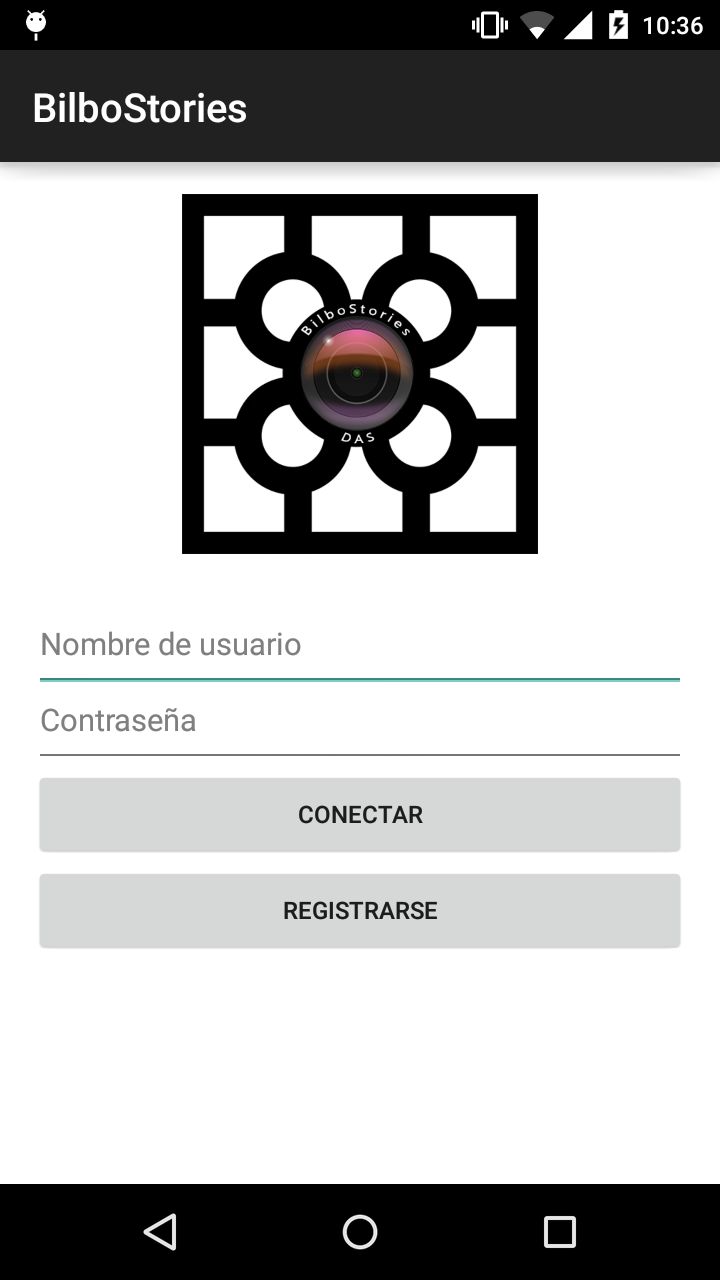
\includegraphics[scale = 0.25 ]{img/0}
		\caption{Log In}
		\label{login1}
	\end{figure}
	
Para poder utilizar la aplicación debemos introducir en los campos correspondientes un nombre de usuario y una contraseña registrados (imagen \ref{login2}) y pulsar el botón Log In.
	
	\begin{figure}[hbtp]
		\centering
		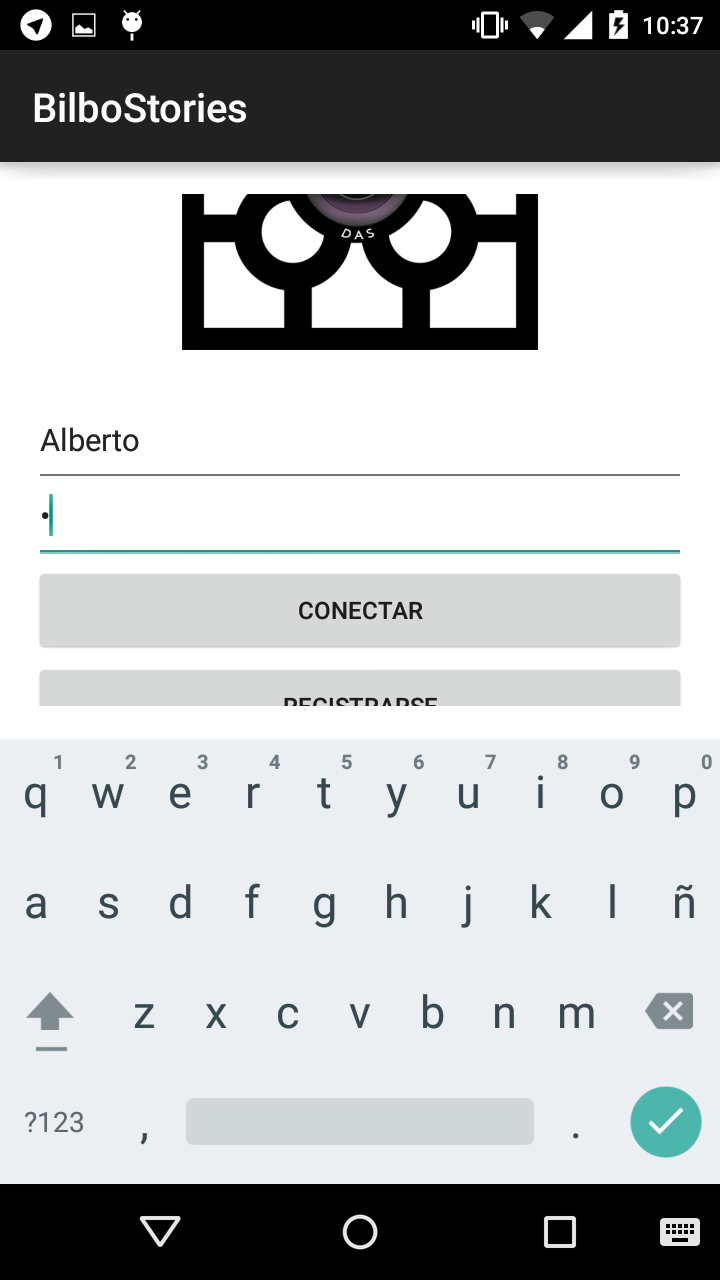
\includegraphics[scale = 0.25 ]{img/1}
		\caption{Log In}
		\label{login2}
	\end{figure}
	
	Si el usuario y contraseña son correctos se nos llevara automáticamente a la Pantalla principal, en caso contrario aparecerá un mensaje de error y tendremos que reintroducir los datos correctos o crear un nuevo usuario pulsando el botón Registrarse.
	
	\FloatBarrier
	\section[Registro]{Registro}
	\label{regis}
	
	Esta pantalla es la que nos permite crear un nuevo usuario para la aplicación (imagen \ref{p14}). 
	
	\begin{figure}[hbtp]
		\centering
		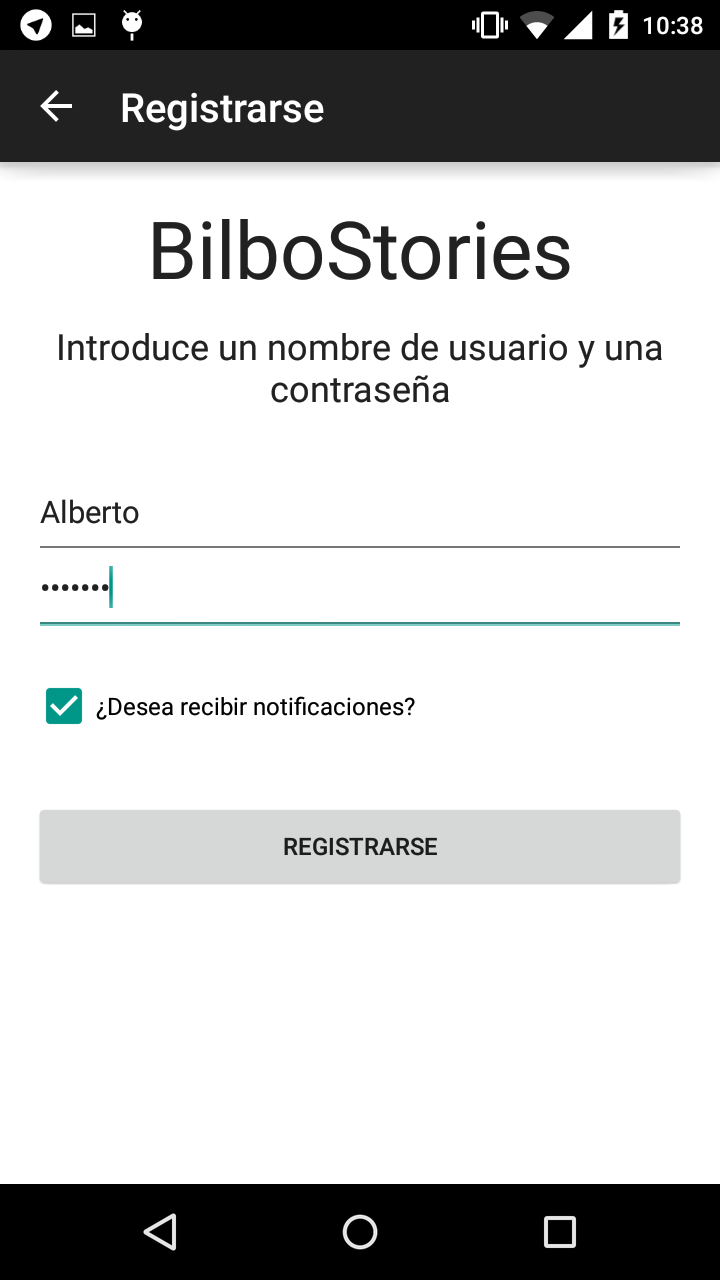
\includegraphics[scale = 0.25 ]{img/2}
		\caption{Registro}
		\label{p14}
	\end{figure}
Cuenta con dos campos donde insertar texto (nombre de usuario y contraseña), un checkbox donde indicar si se desean recibir avisos sobre nuevas publicaciones y un botón para registrar un usuario con los datos introducidos, siendo posible cancelar el proceso pulsando la flecha de la esquina superior izquierda.

Tras introducir los datos y pulsar el botón registrarse retornamos a la pantalla de Log In.
	
	\FloatBarrier
	\section[Pantalla Principal]{Pantalla Principal}
	\label{inPrin}
	
	Esta es la pantalla principal de la aplicación (imagen \ref{p1}), cuenta con un menú lateral que nos permite acceder a las distintas funcionalidades de la aplicación:
	
	\begin{itemize}
		\item Listar las ultimas historias (funcionalidad mostrada por defecto)
		\item Listar las etiquetas que estamos empleando para categorizar las historias
		\item Listar las mejores historias
		\item Modificar datos de la cuenta que estamos utilizando
		\item Cerrar sesión
	\end{itemize}
	
	\begin{figure}[hbtp]
		\centering
		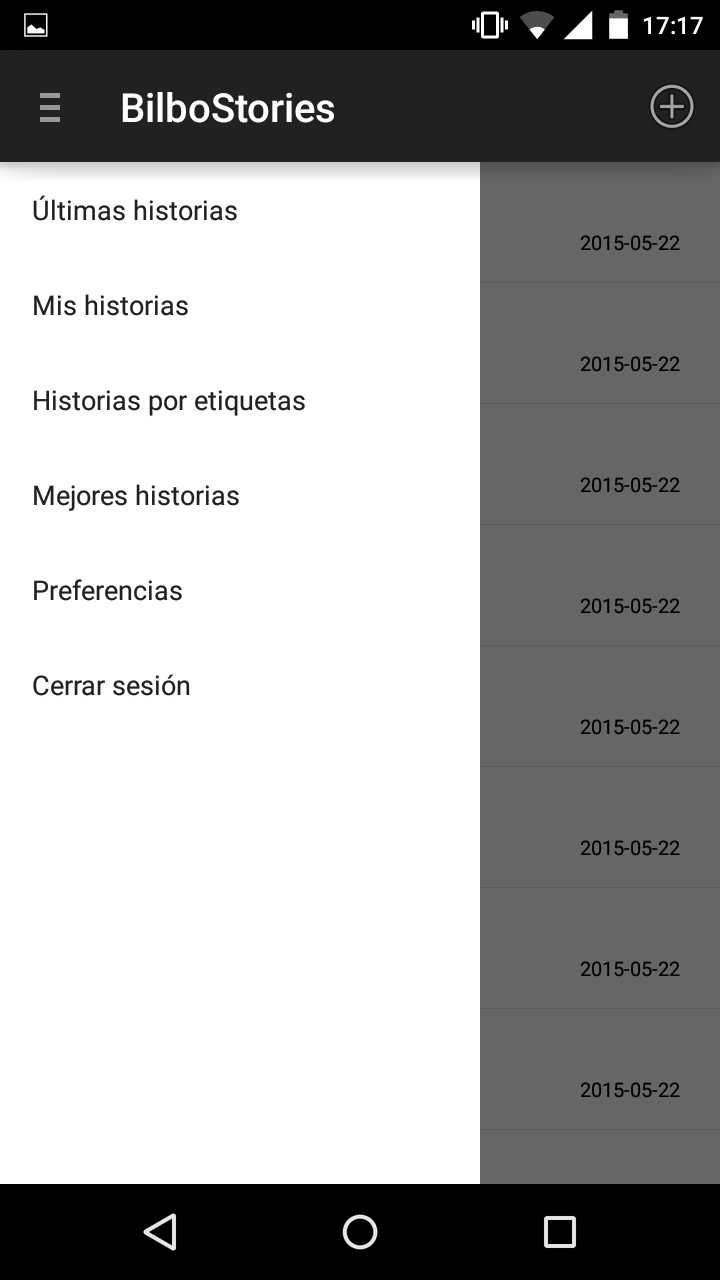
\includegraphics[scale = 0.25 ]{img/3}
		\caption{Pantalla Principal}
		\label{p1}
	\end{figure}
	
	El menú es accesible desde cualquiera de las funcionalidades de listado y la de modificación de preferencias.
	
	\FloatBarrier
	\section[Ultimas Historias]{Ultimas Historias}
	
	Esta funcionalidad es la encargada de mostrarnos las historias que han sido creadas o modificadas más recientemente.
	
	\begin{figure}[hbtp]
		\centering
		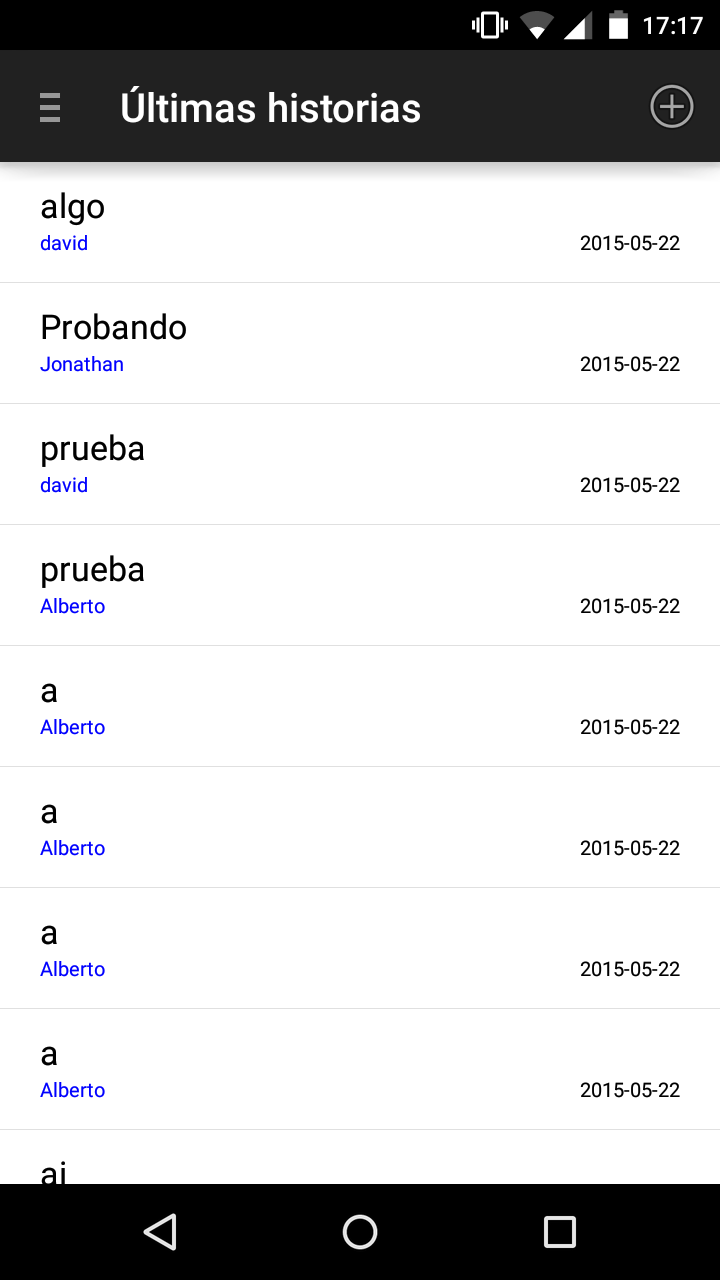
\includegraphics[scale = 0.25 ]{img/4}
		\caption{Ultimas Historias}
		\label{p11}
	\end{figure}
	
	Si pulsamos alguna de las historias de la lista se abrirá una nueva ventana que muestra en detalle la historia seleccionada.
	
	\FloatBarrier
	\section[Mis Historias]{Mis Historias}
	Esta funcionalidad es la encargada de mostrarnos las historias que han sido por el usuario con el que hemos iniciado la aplicación.
	
	\begin{figure}[hbtp]
		\centering
		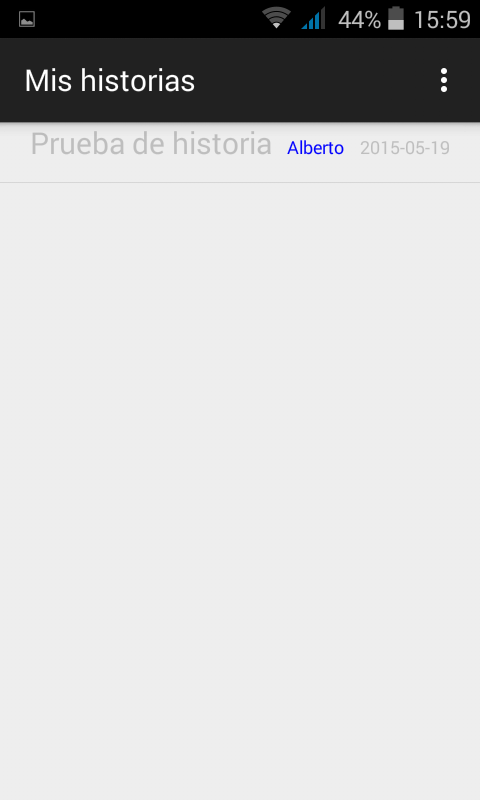
\includegraphics[scale = 0.25 ]{img/5}
		\caption{Mis Historias}
		\label{p12}
	\end{figure}
	
	Si pulsamos alguna de las historias de la lista se abrirá una nueva ventana que muestra en detalle la historia seleccionada.
	
	\FloatBarrier
	\section[Por Etiquetas]{Por Etiquetas}
	
	Esta funcionalidad es la encargada de mostrarnos la lista de etiquetas encargadas para categorizar las historias disponibles, junto al nombre se muestra el número de historias que tienen esa etiqueta asignada.
	
	\begin{figure}[hbtp]
		\centering
		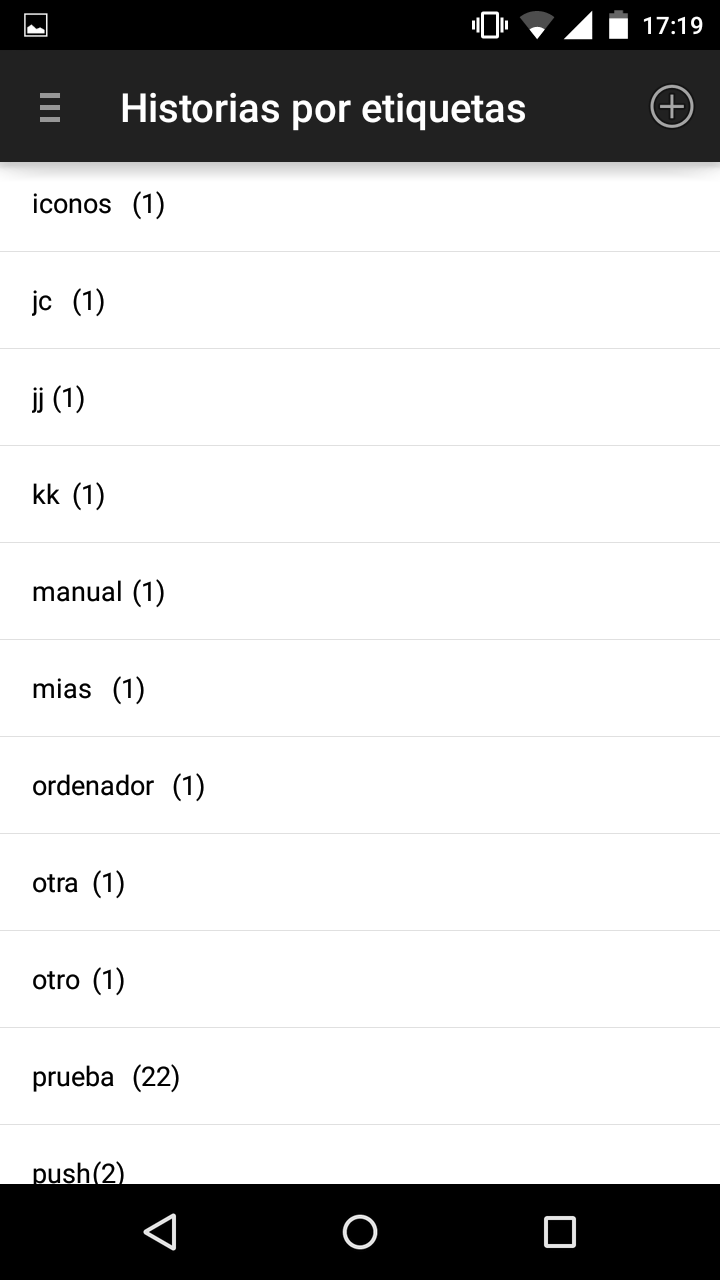
\includegraphics[scale = 0.25 ]{img/6}
		\caption{Por Etiquetas}
		\label{p13}
	\end{figure}
	
	Si pulsamos una de las etiquetas se nos muestra una lista con las historias que tienen la etiqueta pulsada asignada.
	
	\begin{figure}[hbtp]
		\centering
		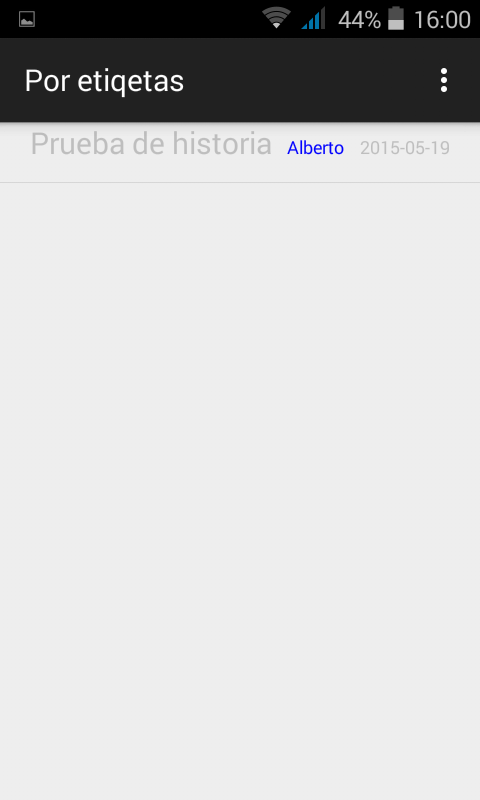
\includegraphics[scale = 0.25 ]{img/7}
		\caption{Por Etiquetas}
		\label{p15}
	\end{figure}
	
	\FloatBarrier
	\section[Mejores]{Mejores}
	
	\FloatBarrier
	\section[Preferencias]{Preferencias}
	
	Esta funcionalidad nos permite modificar la contraseña para el usuario con el que hemos iniciado la aplicación y modificar la opción de recibir avisos sobre nuevas publicaciones.
	
	\begin{figure}[hbtp]
		\centering
		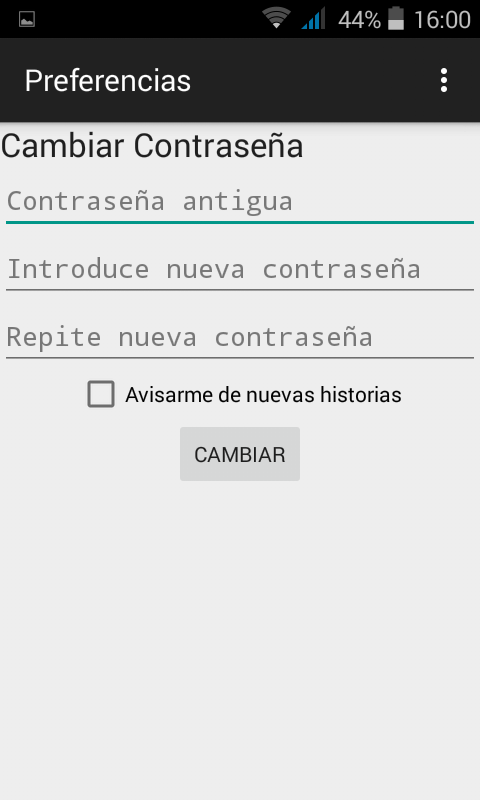
\includegraphics[scale = 0.25 ]{img/9}
		\caption{Preferencias}
		\label{p16}
	\end{figure}
	
	Para ello debemos introducir la antigua contraseñan, dos veces la nueva contraseña, si se desea seleccionar el checkbox de avisos y pulsar el botón cambiar.
	
	\FloatBarrier
	\section[Cerrar Sesión]{Cerrar Sesión}
	Esta funcionalidad nos permite hacer log out de la aplicación y nos lleva a la pantalla de log in para poder iniciar la aplicación con otro usuario. Nos pedirá confirmar la acción para llevarla a cabo. 
	
	
	\FloatBarrier
	\section{Crear historia}
	Esta funcionalidad nos permite crear una historia que todos los usuarios podrán ver. La funcionalidad es accesible desde cualquiera d las funcionalidades mencionadas en la sección \ref{inPrin} a través del icono ``+'' situado en la esquina superior derecha.
	
	Tras acceder se nos muestra la pantalla de la imagen \ref{p17}.
	\begin{figure}[hbtp]
		\centering
		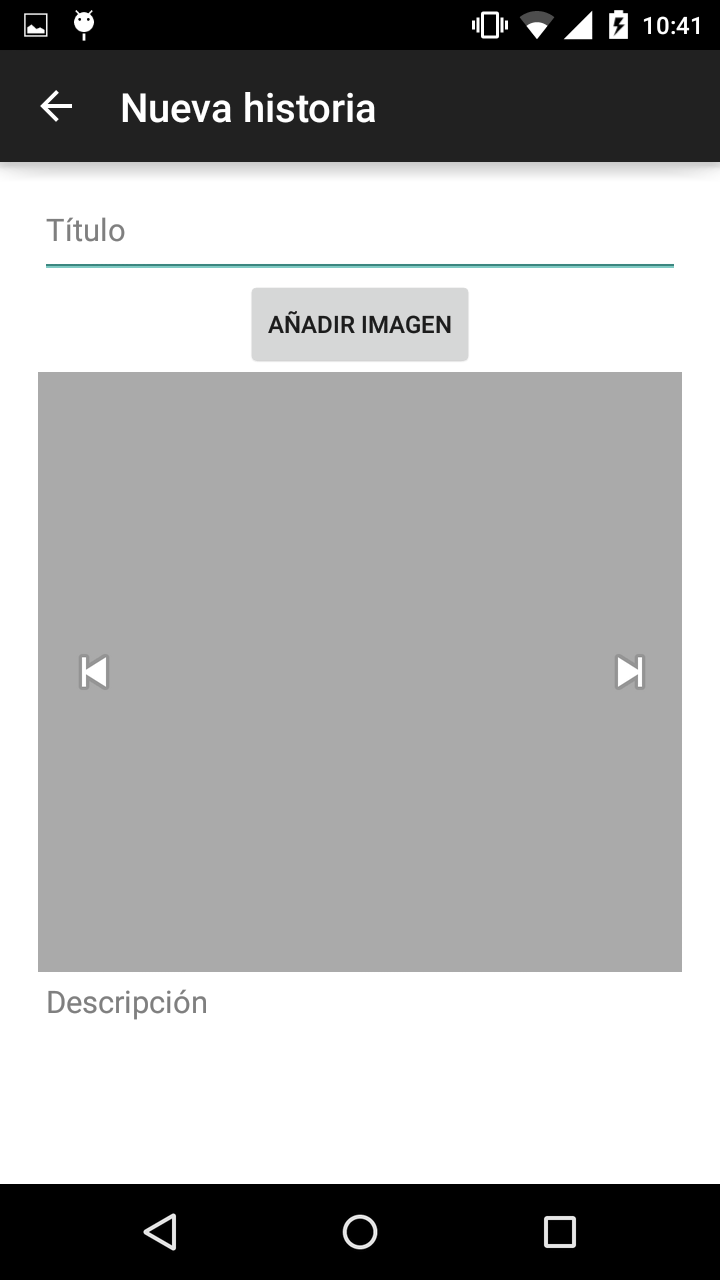
\includegraphics[scale = 0.25 ]{img/10}
		\caption{Crear historia}
		\label{p17}
	\end{figure}
	
	Para subir una historia, es necesario rellenar los campos obligatorios, el título, la descripción y elegir al menos una imagen.
	
	Pulsando en ``Añadir imagen'' se nos muestra el diálogo de la imagen \ref{p18}, que nos da la posibilidad de realizar una foto o seleccionar una imagen de la galería. En cualquier caso, tras elegir una imagen, ésta se añadirá a la historia (ver imagen \ref{p19}). En caso de que hubiera un error, se informaría del problema. Se pueden ver las diferentes imágenes pulsando en los botones laterales de la sección gris.
	
		\begin{figure}[hbtp]
			\centering
			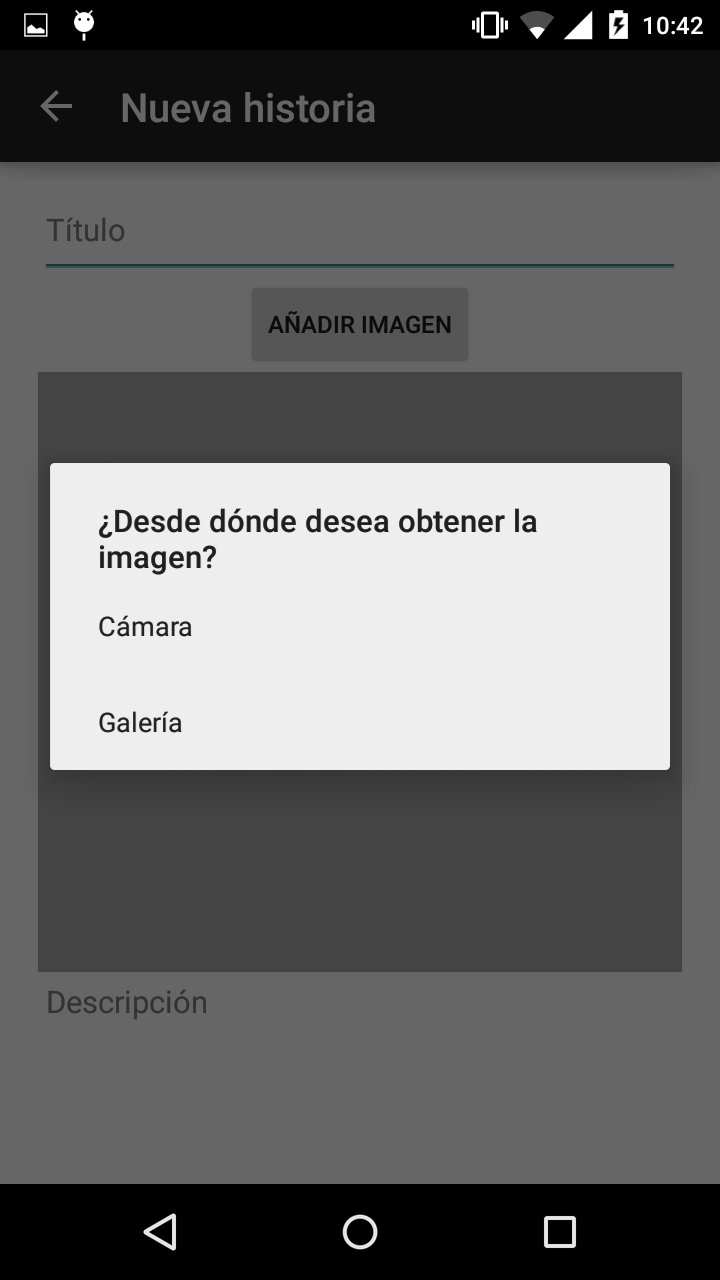
\includegraphics[scale = 0.25 ]{img/12}
			\caption{Selección de fuente de la imagen}
			\label{p18}
		\end{figure}
		
		\begin{figure}[hbtp]
			\centering
			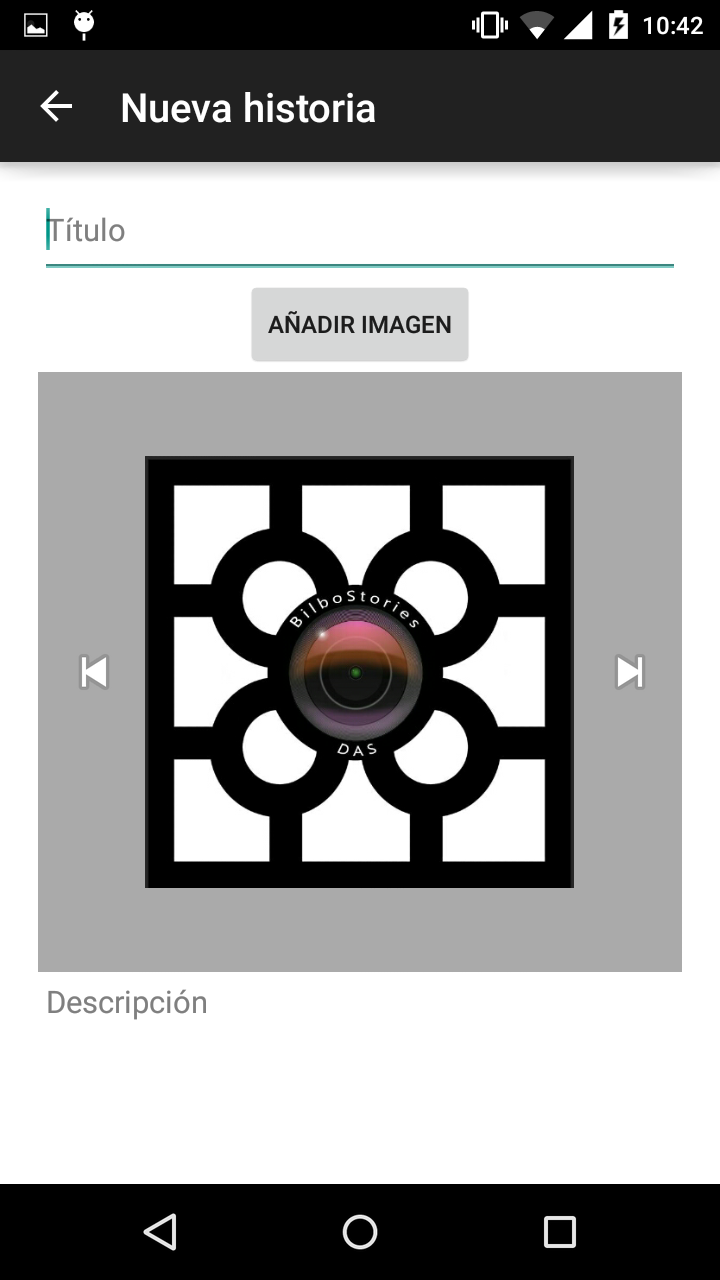
\includegraphics[scale = 0.25 ]{img/13}
			\caption{Selección de fuente de la imagen}
			\label{p19}
		\end{figure}
		
	Las etiquetas de la imagen son opcionales, si queremos especificar varias, cada una debe ir separada por comas, ver imagen \ref{p20}. Una vez completo, pulsamos en ``Crear historia'' y la imagen se guardará en el servidor. En caso de haber algún problema (campos no completos, falta de imágenes, error de subida) se informaría del mismo al usuario.
	
		\begin{figure}[hbtp]
			\centering
			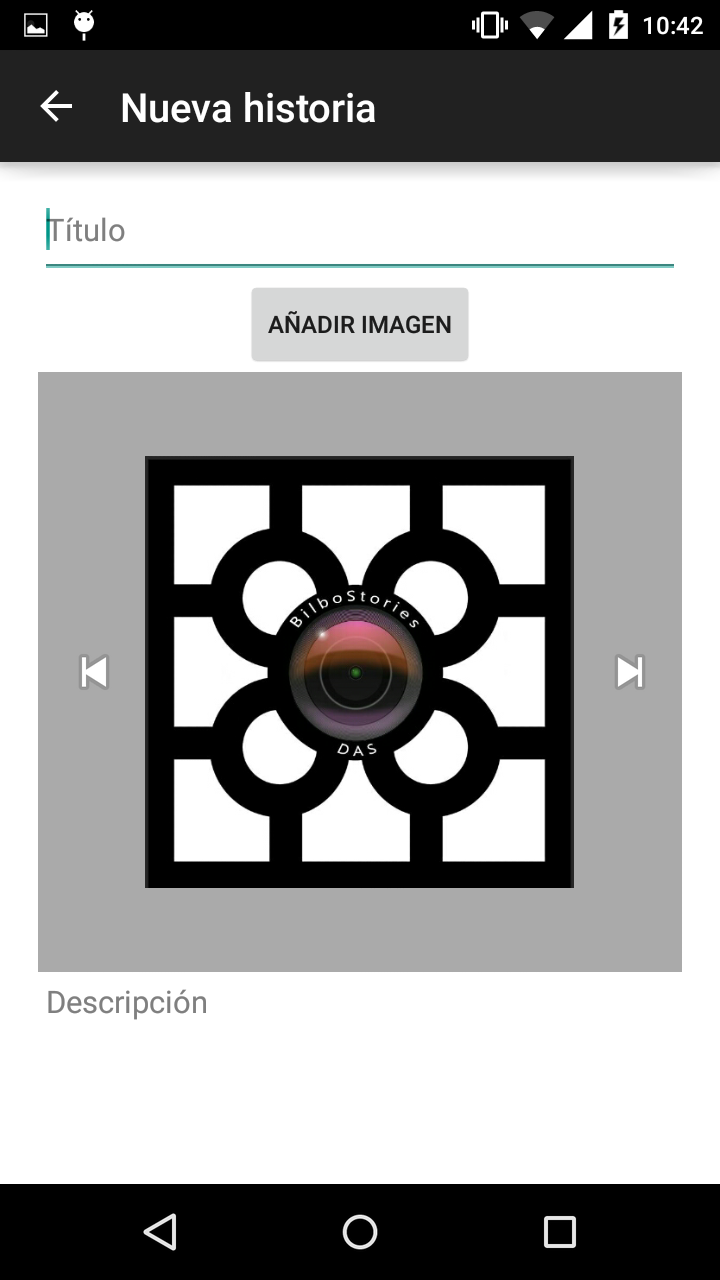
\includegraphics[scale = 0.25 ]{img/13}
			\caption{Especificación de etiquetas en una historia}
			\label{p20}
		\end{figure}
		
	\FloatBarrier
	\section{Notificaciones Push}
	
	En caso de que hayamos marcado la opción en nuestras preferencias, cuando un usuario cree una nueva historia, recibiremos una notificación push en el dispositivo. Pulsándola, accederemos directamente a la historia (imagen \ref{p21}).
	
	\begin{figure}[hbtp]
		\centering
		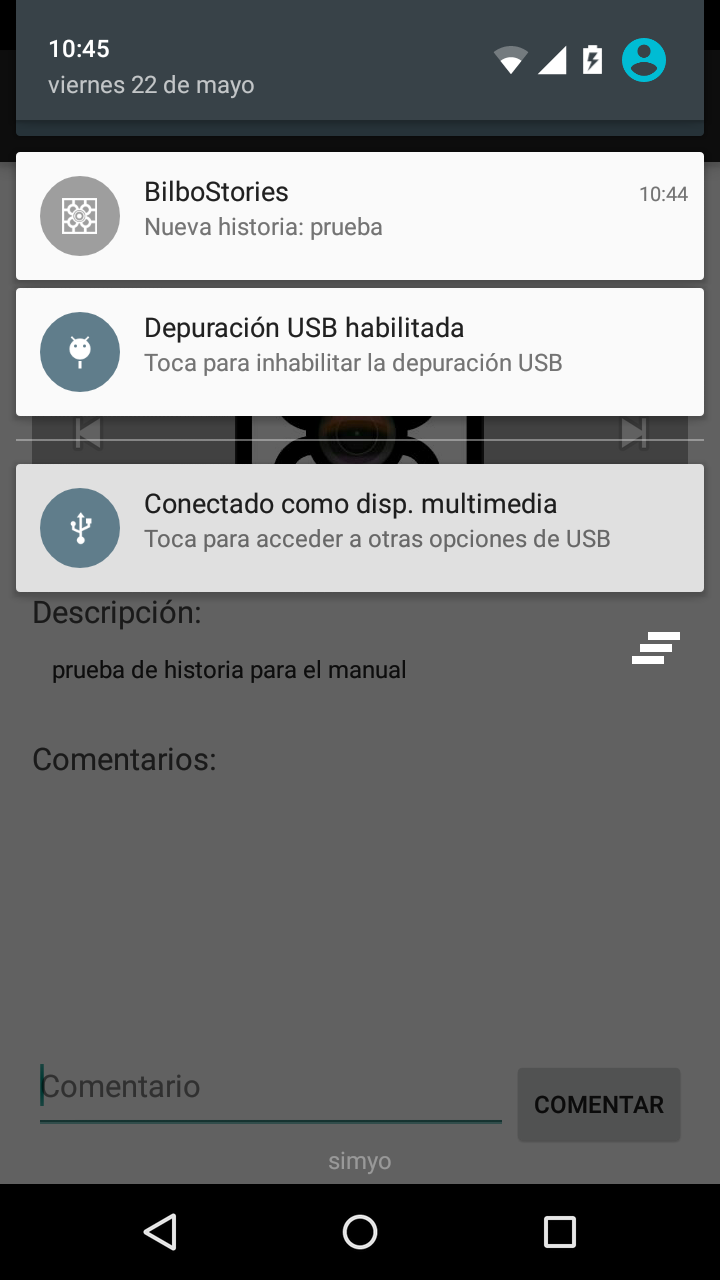
\includegraphics[scale = 0.25 ]{img/16}
		\caption{Notificación de la aplicación}
		\label{p21}
	\end{figure}
	
	También en caso de que se haga un comentario en una historia a la que estemos suscritos recibiremos la notificación.
	
	La suscripción a una historia puede producirse por:
	\begin{itemize}
		\item Crear una historia. Automáticamente el creador queda suscrito.
		\item Comentar una historia. También se suscribe automáticamente y el usuario recibirá notificaciones de nuevos comentarios.
	\end{itemize}
	
	\FloatBarrier
	\section{Ver historia}
	
	Bien accediendo desde uno de los múltiples listados o de una notificación, la pantalla a la que se accede es la de la imagen \ref{p22}.
	
	Se muestra la información de la imagen
	
	\begin{figure}[hbtp]
		\centering
		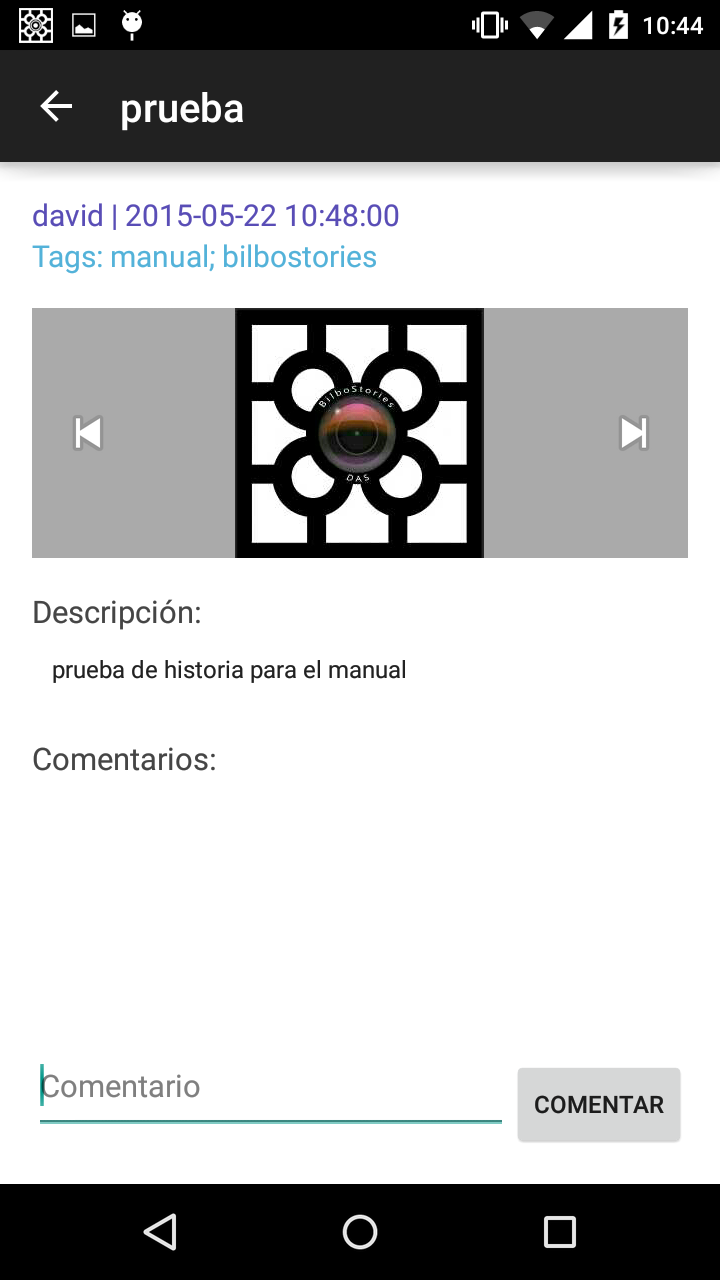
\includegraphics[scale = 0.25 ]{img/15}
		\caption{Vista de una historia}
		\label{p22}
	\end{figure}
	
	\FloatBarrier
	\section{Comentar historias}
	
	Dentro de la vista de la historia, usando el formulario de la parte inferior podemos escribir y enviar el comentario.
	
	Una vez enviado, aparecerá en pantalla (ver imagen \ref{p23}) y los usuarios suscritos, como ya se ha comentado, recibirán una notificación.
	
	\begin{figure}[hbtp]
		\centering
		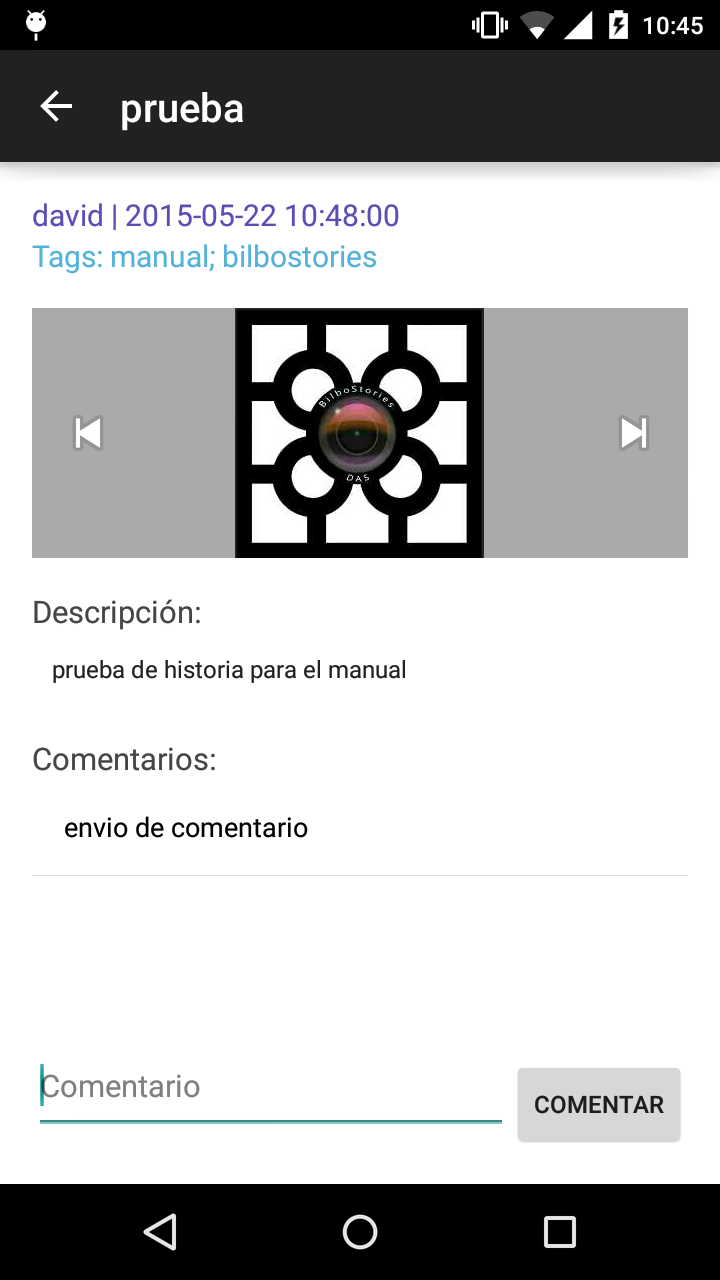
\includegraphics[scale = 0.25 ]{img/17}
		\caption{Historia con el nievo comentario}
		\label{p23}
	\end{figure}
	
	
	
\end{document}